\documentclass[a4paper]{article}
\usepackage{tikz} 
\usepackage{array}
\usepackage{float}
\usepackage{standalone}


\title{}
\author{}
\date{}


\begin{document}

\section{Introduction}
Cultural evolution theories provide a set of methods that can be used to account these dynamic of changes, focused on the production of olive oil amphorae during the Roman Empire. 
To achieve this goal, multivariate methods were used to evaluate the differences on the pattern production among pottery workshops. \\
Specifically we want to identify the origin of these changes and if these changes were produced by cultural reasons depending on the spatial distance and other cultural constraints. As hypothesis, we propose that spatial distribution of pottery workshops is the main influence of the making techniques processes \cite{schillinger}. Four pottery workshops, showed in the map \textbf{(fig.1)} were studied from different spaces in \emph{Baetica}. 
\section{Empirical Studies}
Measure on amphora and PCA : we observe a correlation of variation given distance.


\section{Theoretical Exploration}
\subsection{Experimental Setup}
\begin{figure}[H!]
    \begin{tabular}{m{4cm}m{4cm}}
	{\tiny No Horizontal Transmission} & {\centering\tiny Horizontal Transmission }\\
	\resizebox{4cm}{!}{
	    \documentclass{standalone}

\begin{document}
	    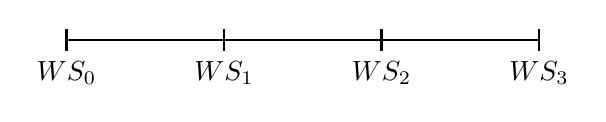
\begin{tikzpicture}[thick,scale=2]
		\coordinate (WS0) at (0,0);
		\coordinate (WS1) at (1,0);
		\coordinate (WS2) at (2,0);
		\coordinate (WS3) at (3,0);
		\draw[thick,-] (0,0) -- (3,0) node[anchor=north west] {};   
		\foreach \x in {0,1,2,3}
		\draw (\x cm,2pt) -- (\x cm,-2pt) node[anchor=north] {$WS_\x$};

	    \end{tikzpicture}
\end{document}



	}
	&
	\resizebox{4cm}{!}{
	    \documentclass{standalone}

\begin{document}
    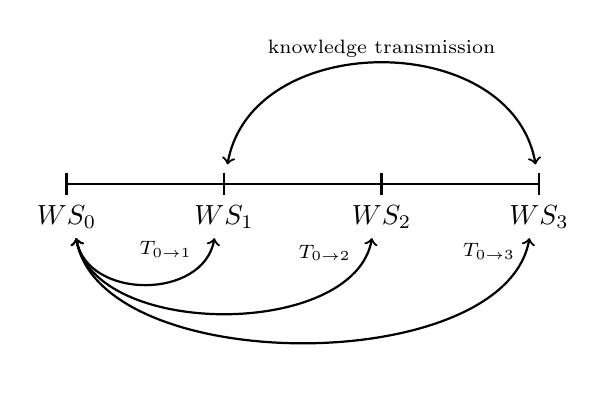
\begin{tikzpicture}[thick,scale=2]
		\coordinate (WS0) at (0,0);
		\coordinate (WS1) at (1,0);
		\coordinate (WS2) at (2,0);
		\coordinate (WS3) at (3,0);
		\draw[thick,-] (0,0) -- (3,0) node[anchor=north west] {};   
		\foreach \x in {0,1,2,3}
		\draw (\x cm,2pt) -- (\x cm,-2pt) node[anchor=north] {$WS_\x$};


		\draw [black,shorten <= 0.25cm, shorten >= 0.25cm, <->] (WS1) to[out=80,in=100,distance=1cm] node[above,font=\scriptsize]{knowledge transmission} (WS3); 


	\draw [black,shorten <= 0.7cm, shorten >= 0.7cm, <->] (WS0) to[out=-80,in=-100,distance=.75cm	]  node[font=\scriptsize,pos=.60	,above]{$T_{0 \rightarrow 1}$} (WS1);
	\draw [black,shorten <= 0.7cm, shorten >= 0.7cm, <->] (WS0) to[out=-80,in=-100,distance=1cm	]  node[font=\scriptsize,pos=.75	,above]{$T_{0 \rightarrow 2}$}(WS2);
	\draw [black,shorten <= 0.7cm, shorten >= 0.7cm, <->] (WS0) to[out=-80,in=-100,distance=1.25cm	]  node[font=\scriptsize,pos=.82		,above]{$T_{0 \rightarrow 3}$}(WS3);

    \end{tikzpicture}

\end{document}


	}\\
	\resizebox{4cm}{!}{
	    \documentclass{standalone}

\begin{document}
	    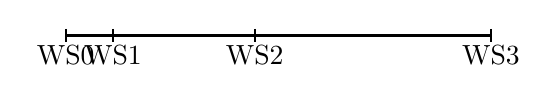
\begin{tikzpicture}[thick,scale=.6]
		\coordinate (WS0) at (0,0);
		\coordinate (WS1) at (1,0);
		\coordinate (WS2) at (4,0);
		\coordinate (WS3) at (9,0);
		\draw[thick,-] (0,0) -- (9,0) node[anchor=north west] {};   
		\foreach \x in {0,1,4,9}
		\draw (\x cm,4pt) -- (\x cm,-4pt) node[anchor=north] {};
		\draw (WS0) node[anchor=north]{WS0};
		\draw (WS1)node[anchor=north]{WS1};
		\draw (WS2)node[anchor=north]{WS2};
		\draw (WS3)node[anchor=north]{WS3};
	    \end{tikzpicture}
\end{document}


	}	&
	\resizebox{4cm}{!}{
	    
\documentclass{standalone}

\begin{document}
	    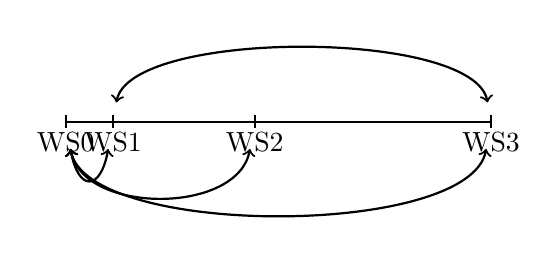
\begin{tikzpicture}[thick,scale=.6]
		\coordinate (WS0) at (0,0);
		\coordinate (WS1) at (1,0);
		\coordinate (WS2) at (4,0);
		\coordinate (WS3) at (9,0);
		\draw[thick,-] (0,0) -- (9,0) node[anchor=north west] {};   
		\foreach \x in {0,1,4,9}
		\draw (\x cm,4pt) -- (\x cm,-4pt) node[anchor=north] {};
		\draw (WS0) node[anchor=north]{WS0};
		\draw (WS1)node[anchor=north]{WS1};
		\draw (WS2)node[anchor=north]{WS2};
		\draw (WS3)node[anchor=north]{WS3};

		\draw [black,shorten <= 0.25cm, shorten >= 0.25cm, <->] (WS1) to[out=80,in=100,distance=2cm] (WS3); 
		\draw [black,shorten <= .35cm, shorten >= .35cm, <->] (WS0) to[out=-80,in=-100,distance=1.5cm	]  (WS1);
		\draw [black,shorten <= .35cm, shorten >= .35cm, <->] (WS0) to[out=-80,in=-100,distance=2cm	]  (WS2);
		\draw [black,shorten <= .35cm, shorten >= .35cm, <->] (WS0) to[out=-80,in=-100,distance=2.5cm	]  (WS3);
	    \end{tikzpicture}
\end{document}


	}	
    \end{tabular}
\end{figure}


\subsection{Results}
    \begin{figure}[H!]
	\begin{tabular}{m{4cm}m{4cm}}
	    {\tiny \hspace{.4cm}No Horizontal Transmission} & {\centering\tiny Horizontal Transmission }\\
	    \includegraphics[height=4cm]{images/lineNC.png}
	    &
	    \includegraphics[height=4cm]{images/lineC.png}\\
	    \includegraphics[height=4cm]{images/cubeNC.png}
	    &
	    \includegraphics[height=4cm]{images/cubeC.png}\\
	\end{tabular}
	\caption{Evolution of the varation between the workshop of the mean of the exterior diameter}
    \end{figure}
 


\end{document}




